\chapter{Analisis}
\label{chap:analisis}
Bab ini membahas tentang analisis dari SharIF-Judge yang digunakan oleh Teknik Informatika. SharIF-Judge memiliki fungsi utama yaitu untuk mengevaluasi kode program yang telah dikumpulkan oleh pengguna secara otomatis. SharIF-Judge digunakan pada beberapa matak kuliah pemrograman Teknik Informatika Unpar untuk mempermudah evaluasi yang akan dilakukan oleh pengajar.

\section{SharIF-Judge}
\label{sec: SharIF-Judge}
Sharif Judge adalah online judge gratis untuk bahasa pemrograman C, C++, Java dan Python \cite{sharif_judge}. Perangkat lunak ini diciptakan oleh Mohammad Javad Naderi pada tahun 2014 dan bersifat open source. Antarmuka Sharif Judge ditulis menggunakan bahasa pemrograman PHP (framework CodeIgniter) dan backend menggunakan BASH.
erikut ini merupakan fitur-fitur yang dimiliki oleh Sharif Judge antara lain yaitu:
\begin{itemize}
    \item {\textit{Multiple Role}}\newline
        Pada SharIF-Judge, \textit{User} memiliki 4 jenis \textit{role} yang dibedakan berdasarkan level, dimana level tersebut digunakan untuk memisahkan aksi yang dapat dilakukan setiap \textit{role}. 4 \textit{role} tersebut adalah \textit{Admin}, \textit{Head Instructor}, \textit{Instructor}, dan \textit{Student}. 
        
    \begin{table}[H] %atau h saja untuk "kira kira di sini"
	    \centering 
	    \caption{Tabel \textit{role}}
	    \label{tab:level}
	    \begin{tabular}{|c|c|}
		    \hline
		    \textit{Role} & Level \\
		    \hline
		    \textit{Admin} & 3 \\
		    \hline
		    \textit{Head Instructor} & 2 \\
		    \hline
		    \textit{Instructor} & 1 \\
		    \hline
		    \textit{Student} & 0 \\
		    \hline
	    \end{tabular} 
    \end{table}
    
        Pada Tabel \ref{tab:level} menunjukan level role yang ada pada SharIF-Judge. Setiap \textit{role} tersebut, dapat melakukan aksi yang berbeda-beda yang disesuaikan dengan level role. Untuk melihat aksi apa saja yang dapat dilakukan setiap \textit{role} dapat dilihat pada Tabel \ref{tab:aksi}.
    \begin{table}[H]
	    \centering 
	    \caption{Tabel \textit{Action}}
	    \label{tab:aksi}
	    \begin{tabular}{|c|c|c|c|c|}
		    \hline
		    \textit{Action} & \textit{Admin} & \textit{Head Instructor} & \textit{Instructor} & \textit{Student} \\
		    \hline
		    Mengubah \textit{Setting} & O & X & X & X \\
		    \hline
		    Menambah/Menghapus \textit{User} & O & X & X & X \\
		    \hline
		    Mengubah \textit{role users} & O & X & X & X \\
		    \hline
		    Menambah/Menghapus/Mengubah \textit{Assignment} & O & O & X & X \\
		    \hline
		    Mengunduh \textit{Test} & O & O & X & X \\
		    \hline
		    Menambah/Menghapus/Mengubah Notifikasi & O & O & X & X \\
		    \hline
		    Rejudge & O & O & X & X \\
		    \hline
		    Melihat/Pause/Melanjutkan/Submission Queue & O & O & X & X \\
		    \hline
		    Mendeteksi Kode yang Mirip  & O & O & X & X \\
		    \hline
		    Melihat Semua Kode  & O & O & O & X \\
		    \hline
		    Mengunduh Kode Final  & O & O & O & X \\
		    \hline
		    Memilih \textit{Assignment}   & O & O & O & O \\
		    \hline
		    Submit  & O & O & O & O \\
		    \hline
	    \end{tabular} 
    \end{table}
        Pengguna dapat menambahkan \textit{user} dengan menggunakan fitur \textit{Add User} pada halaman \textit{User}, Pengguna harus mengisi semua informasi yang ada pada text area. Baris dimulai dengan komentar
\#. Setiap baris lainnya mewakili pengguna dengan sintaks berikut:

     \begin{lstlisting}[basicstyle=\ttfamily, frame=single,
        columns=fullflexible, breaklines=true, numbers=none]
USERNAME EMAIL PASSWORD ROLE
- Username dapat berisikan huruf kecil atau nomor dan harus terdiri antara 3 
  sampai 20 karakter.
- Password harus terdiri antara 6 sampai 30 karakter.
- Pengguna dapat menggunakan RANDOM[n] untuk menghasilkan password acak yang terdiri dari n-digit karakter.
- ROLE harus terdiri dari salah satu yang disebutkan sebagai berikut: `admin', `head_instructor', `instructor', dan `student'
    \end{lstlisting}
    
    Berikut ini adalah contoh penggunaan sintaks untuk \textit{add user}:
 \begin{lstlisting}[basicstyle=\ttfamily, frame=single,
    columns=fullflexible, breaklines=true, numbers=none]
# This is a comment!
# This is another comment!
instructor instructor@sharifjudge.ir 123456 head_instructor
instructor2 instructor2@sharifjudge.ir random[7] instructor
student1 st1@sharifjudge.ir random[6] student
student2 st2@sharifjudge.ir random[6] student
student3 st3@sharifjudge.ir random[6] student
student4 st4@sharifjudge.ir random[6] student
student5 st5@sharifjudge.ir random[6] student
student6 st6@sharifjudge.ir random[6] student
student7 st7@sharifjudge.ir random[6] student
    \end{lstlisting}

    \item \textit{Sandboxing}\newline
        \textit{Sandboxing} adalah sebuah mekanisme dimana sebuah aplikasi yang dikirimkan oleh pengguna, dapat dijalankan dalam lingkungan virtual yang aman dan menghindari adanya serangan keluar dari Sharif Judge. \\
        
    \item \textit{Cheat Detection}
    
    \textit{Cheat Detection} berguna sebagai pendeteksi adanya kode yang mirip dan sebagai pendeteksi kecurangan. Untuk pengecekan digunakan \textit{Moss}(\textit{Measure Of Software Similarity}) Moss adalah perangkat lunak yang digunakan oleh guru dan penerbit untuk menemukan plagiarisme perangkat lunak. Perangkat lunak ini dikembangkan oleh Stanford, dan telah menjadi alat utama untuk memeriksa plagiarisme kode. MOSS diciptakan untuk menghentikan kelaziman pada siswa untuk menyalin kode dan langsung selesai tanpa adanya pengertian dari siswa terhadap pelajaran tersebut\cite{moss} \\
    \item Penilaian berbeda untuk keterlambatan pengumpulan
    
    Hal ini berguna agar jika pelajar ada yang membutuhkan pengertian khusus dan memiliki alasan yang baik, pengajar dapat memberikan pengecualian dan memberikan hukuman ringan.\\
    \item Antrian pengiriman \newline
    Hal ini berguna agar Sharif Judge tidak \textit{down} akibat banyaknya pengiriman.\\
    
    \item Mengunduh nilai dalam bentuk \textit{excel}\newline
    Hal ini berguna agar pengajar tidak mendapatkan kesulitan untuk menyimpan data nilai pelajar.\\
    
    \item Mengunduh kode yang dikumpulkan dalam bentuk zip \newline
    Hal ini berguna agar ketika kode yang harus dikumpulkan ada banyak dan ketika pengajar ingin memeriksa, file tersedia dengan rapih. \\
    
    \item Metode "Output Comparison" dan "Tester Code" untuk memeriksa \textit{output}. \newline
    Hal ini berguna agar pelajar mengetahui apakah pekerjaan yang dikirimkan tersebut sudah benar atau masih kurang tepat. \\
    
    \item Penilaian ulang \newline
    Hal ini berguna agar ketika pengajar melakukan kesalahan penilaian, pengajar dapat melakukan edit. \\
    \item Papan nilai\newline
    Hal ini berguna agar pelajar dapat melihat nilai dari pelajar-pelajar yang lain dan bisa menjadi motivasi bagi pelajar tersebut. \\
    \item Notifikasi \newline
    hal ini berguna agar ketika ada tugas yang harus dikumpulkan, pelajar mengetahuinya dan tidak terlewat.
\end{itemize}

\subsection{Instalasi}
\label{sec:Instalasi}
Untuk dapat menjalankan Sharif Judge, diwajibkan untuk memiliki server Linux dan mengikuti tahapan sebagai berikut\footnote{\url{https://github.com/mjnaderi/Sharif-Judge}\label{github}}:
\begin{itemize}
    \item Menjalankan PHP versi 5.3 atau versi yang lebih baru.
    \item Pengguna dapat menjalankan PHP dari command line  dan pengguna perlu menginstall paket PHP CLI.
    \item Memiliki \textit{Mysql} atau \textit{PostgreSql databse}.
    \item PHP memiliki akses untuk menjalankan perintah \textit{shell} terutama untuk fungsi \textit{shell\_exec}. contohnya seperti \textit{command} di bawah ini: 
    
     \begin{lstlisting}[basicstyle=\ttfamily, frame=single,
    columns=fullflexible, breaklines=true, numbers=none]
echo shell_exec(``php -v'');
    \end{lstlisting}
    
    \item Untuk melakukan proses kompilasi dan menjalankan kode yang dikumpulkan adalah (\textit{gcc, g++, javac, java, python2, python3 commands})
    \item Disarankan untuk melakukan instalasi \textit{Perl} dengan alasan agar memiliki ketepatan waktu, penggunaan \textit{memory} yang terbatas dan memaksimalkan batas ukuran pada \textit{output} kode yang dikirimkan.
\end{itemize}
Jika persyaratan diatas telah selesai dilakukan, dapat melakukan instalasi sebagai berikut: 
\begin{itemize}
    \item Mengunduh versi terakhir dari Sharif Judge dan unpack file yang berhasil diunduh, letakan pada direktori html publik
    \item Untuk mempermudah pindahkan folder \textit{system}  dan \textit{application} keluar dari direktori publik dan masukan \textit{path} lengkap pada file index.php

     \begin{lstlisting}[basicstyle=\ttfamily, frame=single,
    columns=fullflexible, breaklines=true, numbers=none]
        $system_path = `/home/mohammad/secret/system`;
        $application_folder = `/home/mohammad/secret/application`;
    \end{lstlisting}

    \item Membuat sebuah \textit{Mysql} atau \textit{PostgreSql database} untuk Sharif Judge.
    \item Mengatur koneksi database di file application/config/database.php.

 \begin{lstlisting}[basicstyle=\ttfamily, frame=single,
    columns=fullflexible, breaklines=true, numbers=none]
/* Enter database connection settings here: */
`dbdriver' => `postgre', // database driver (mysqli, postgre)
`hostname' => `localhost', // database host
`username' => `, // database username
`password' => `, // database password
`database' => `, // database name
`dbprefix' => `shj_', // table prefix
/**********************************************/
    \end{lstlisting}


    \item Membuat direktori application/cache/Twig agar dapat ditulis oleh PHP
    \item Membuka halaman utama Sharif Judge pada web browser \item \textit{Log in}  menggunakan akun \textit{admin}
    \item Memindahkan folder \textit{tester} dan \textit{assigments} di luar direktori publik lalu simpan \textit{path} lengkap pada halaman \textit{Settings} . Dua folder tersebut harus dapat ditulis oleh PHP. File-file yang diunggah akan disimpan di folder \textit{assigments} sehingga tidak dapat diakses publik.
\end{itemize}

\subsection{\textit{Add Assignment}}
\label{sec: Add Assignment}
Pengguna dapat menambahkan \textit{assignment} dengan cara mengklik menu \textit{Assignments} lalu klik \textit{add} pada halaman tersebut\footref{github}. Pada Gambar \ref{fig:addAssignment} merupakan halaman \textit{add assignment}.
 \begin{figure}[h!]
     \centering
     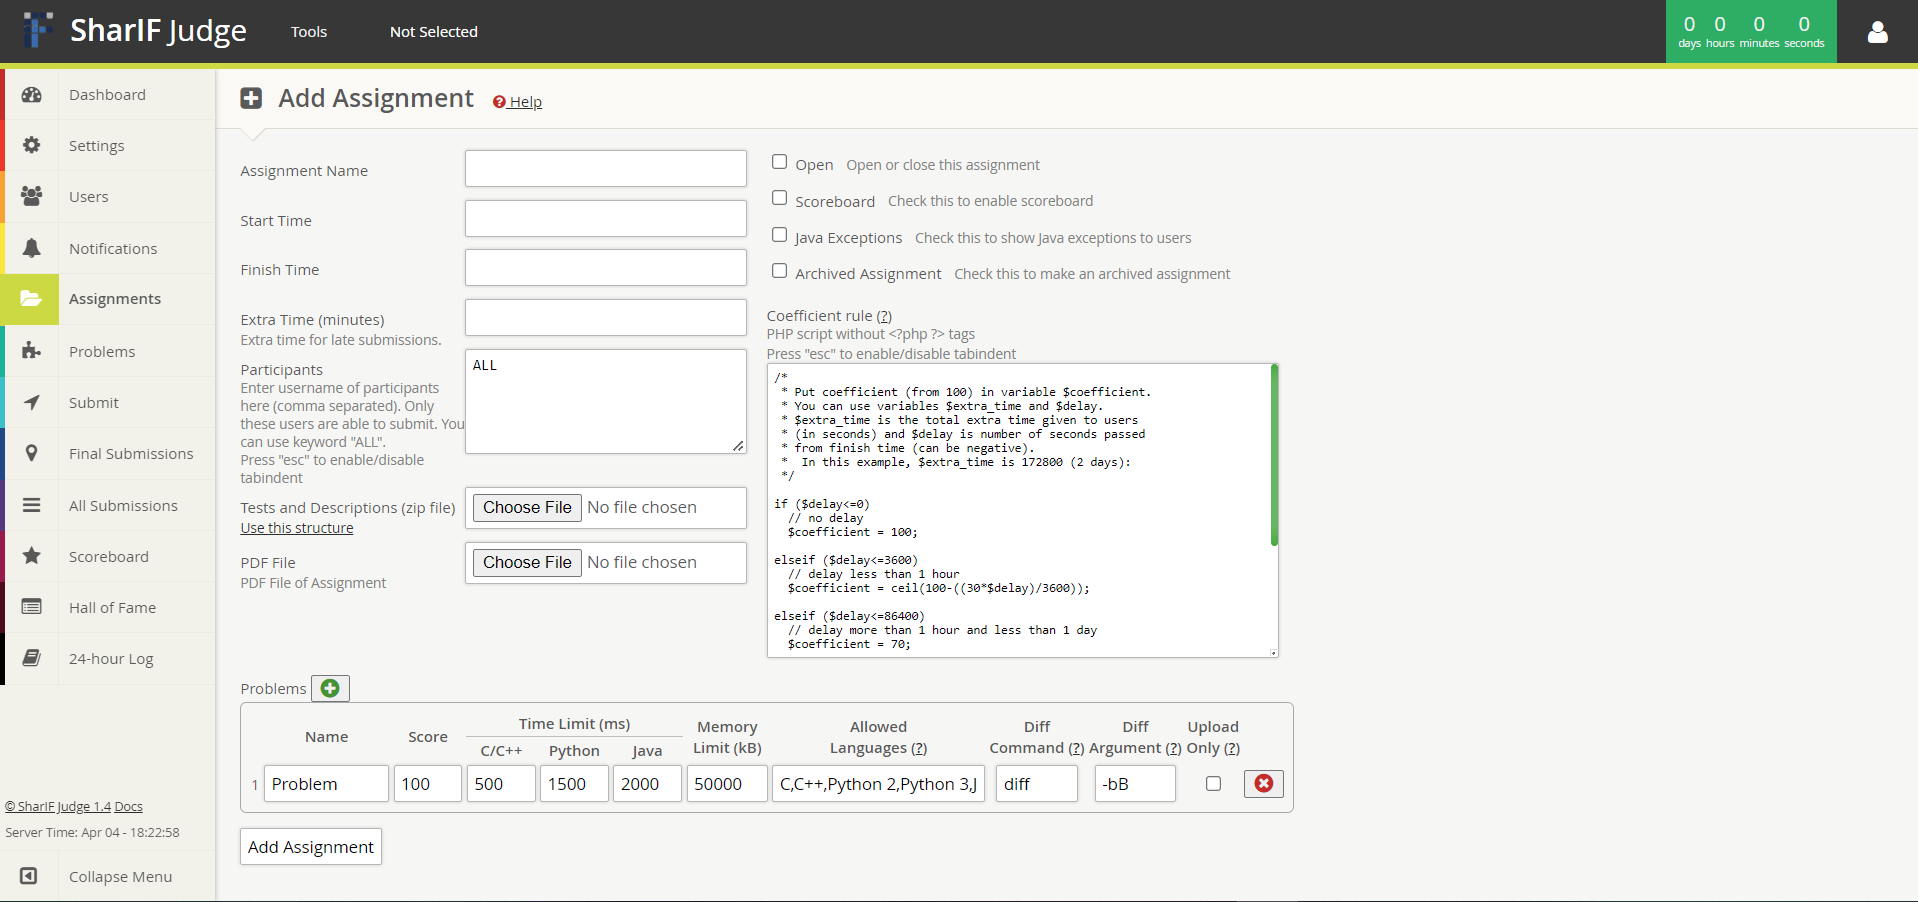
\includegraphics[width=1\linewidth]{Gambar/Add Assignment.PNG}
     \caption{Halaman \textit{Assignment}}
     \label{fig:addAssignment}
 \end{figure}
Berikut ini merupakan pengaturan yang terdapat pada \textit{add assignment}: 
\begin{itemize}
    \item \textit{Assignment Name}\newline
    Memberikan nama pada \textit{assignment} yang akan dibuat \\
    \item \textit{Start Time}\newline
    Menentukan dimulainya waktu dari \textit{assignment} tersebut dan peserta tidak dapat mengumpulkan \textit{assignment} tersebut lebih cepat dari \textit{start time}. Format yang digunakan untuk \textit{start time} adalah \textit{MM/DD/YYYY HH:MM:SS}. Contoh penulisannya adalah 08/31/2013 12:00:00 \\
    \item \textit{Finish Time and Extra Time}\newline
    Peserta tidak dapat melakukan aksi \textit{submit} setelah \textit{Finish time + Extra time}. \textit{Assignment} yang telat akan dikalikan dengan koefisien yang sudah ditentukan. Pengguna harus menulis \textit{script} dalam bahasa PHP untuk menghitung koefisien pada bidang "\textit{Coefficient Rule}". Format yang digunakan dalam pengaturan \textit{finish time} adalah \textit{MM/DD/YYYY HH:MM:SS}. Contoh penulisannya adalah 08/31/2013 23:59:59. "Extra Time" akan terhitung dalam satuan menit. Pengguna juga dapat menggunakan operator aritmatika seperti *, -, +, /. Contoh 120 (2 jam) atau 48*60 (2 hari).\\
    \item \textit{Participants} \newline
    Pengaturan ini berfungsi untuk membatasi peserta yang dapat mengumpulkan assignment. Pengguna dapat menggunakan kata kunci \textit{ALL} pada kolom \textit{Participants} untuk mengijinkan seluruh peserta agar dapat mengumpulkan \textit{assignment}. Untuk membatasi peserta tertentu, pengguna dapat memasukan username peserta pada kolom \textit{Participants}. Setiap username dapat dipisahkan menggunakan tanda koma. Contoh: admin, instructor1, instructor2, student1.\\
    \item \textit{Tests}\newline
    Pengguna dapat mengirim tes kasus dalam \textit{file} zip dengan syarat saat menambahkan tugas, Pengguna harus menyediakan file zip yang berisi kasus uji. File zip ini harus berisi folder untuk setiap masalah (masalah Upload-Only tidak memerlukan folder apa pun). Nama folder harus p1, p2, p3, \ldots Metode yang dapat digunakan untuk memeriksa keluaran setiap masalah adalah dengan metode “Perbandingan \textit{Input/Output}” dan metode “\textit{Tester}”.
    \begin{itemize}
        \item Perbandingan \textit{Input/Output} \newline
        Dalam metode ini, Pengguna harus meletakkan beberapa file \textit{input} dan \textit{output} di folder masalah. SharIF-Judge memberikan setiap file input tes ke kode pengguna dan membandingkan output pengguna dengan output tes. File input harus di folder in dengan nama input1.txt, input2.txt, \ldots dan file output harus di folder out dengan nama output1.txt, output2.txt, \ldots
        \item \textit{Tester}\newline
        Dalam metode ini, Pengguna harus menyediakan beberapa file pengujian input dan file C++ (tester.cpp) dan (opsional) beberapa file pengujian output. SharIF-Judge memberikan file tes input ke kode pengguna dan mendapatkan output pengguna. Kemudian tester.cpp mendapatkan input tes, output tes, dan output pengguna. Jika output pengguna benar, mengembalikan 0, jika tidak mengembalikan 1.
        Pengguna dapat menggunakan template kode ini untuk menulis tester.cpp: 
        
         \begin{lstlisting}[basicstyle=\ttfamily, frame=single,
    columns=fullflexible, breaklines=true, numbers=none]
/*
 * tester.cpp
 */
 #include <iostream>
#include <fstream>
#include <string>
using namespace std;
int main(int argc, char const *argv[])
{
 	ifstream test_in(argv[1]);  /* This stream reads from test's input file  */
	ifstream test_out(argv[2]); /* This stream reads from test's output file */
	ifstream user_out(argv[3]); /* This stream reads from user's output file */
 
	/* Your code here */
	/* If user's output is correct, return 0, otherwise return 1       */
 	...
 }
    \end{lstlisting}

        Diberikan contoh dari file tes kasus dengan struktur file sebagai berikut:
        
         \begin{lstlisting}[basicstyle=\ttfamily, frame=single,
    columns=fullflexible, breaklines=true, numbers=none]
.
|-- p1
|   |-- in
|   |   |-- input1.txt
|   |   |-- input2.txt
|   |   |-- input3.txt
|   |   |-- input4.txt
|   |   |-- input5.txt
|   |   |-- input6.txt
|   |   |-- input7.txt
|   |   |-- input8.txt
|   |   |-- input9.txt
|   |   |-- input10.txt
|   |-- out
|   |   |-- output1.txt
|   |-- tester.cpp
|-- p2
    |-- in
    |   |-- input1.txt
    |   |-- input2.txt
    |   |-- input3.txt
    |   |-- input4.txt
    |   |-- input5.txt
    |   |-- input6.txt
    |   |-- input7.txt
    |   |-- input8.txt
    |   |-- input9.txt
    |   |-- input10.txt
    |-- out
        |-- output1.txt
        |-- output2.txt
        |-- output3.txt
        |-- output4.txt
        |-- output5.txt
        |-- output6.txt
        |-- output7.txt
        |-- output8.txt
        |-- output9.txt
        |-- output10.txt   
    \end{lstlisting}
    \end{itemize}
    
        \item \textit{Open} \newline
        Pengguna dapat membuka atau menutup \textit{assignment} menggunakan pilihan ini. Jika pengguna menutup \textit{assignment}, \textit{non-student users} masih dapat mengumpulkan \textit{assignment}. \\
        \item \textit{Scoreboard} \newline
        Pengguna dapat mengaktifkan atau mematikan papan nilai dengan menggunakan pilihan ini.
        \item \textit{Java Exceptions} \newline
        Pengguna dapat mengaktifkan dan mematikan java exceptions yang ditunjukan kepada \textit{role students}. Perubahan pada pilihan ini tidak berdampak pada kode yang sebelumnya sudah dinilai. Nama \textit{exception} akan muncul ketika pada file pathtester/java\_exceptions\_list berisikan nama \textit{exception} tersebut. Berikut hasil exception yang ditunjukan jika pengguna mengaktifkan pengaturan \textit{Java Exceptions}:
        
         \begin{lstlisting}[basicstyle=\ttfamily, frame=single,
    columns=fullflexible, breaklines=true, numbers=none]
Test 1
ACCEPT
Test 2
Runtime Error (java.lang.ArrayIndexOutOfBoundsException)
Test 3
Runtime Error (java.lang.ArrayIndexOutOfBoundsException)
Test 4
ACCEPT
Test 5
ACCEPT
Test 6
ACCEPT
Test 7
ACCEPT
Test 8
Runtime Error (java.lang.ArrayIndexOutOfBoundsException)
Test 9
Runtime Error (java.lang.StackOverflowError)
Test 10
Runtime Error (java.lang.ArrayIndexOutOfBoundsException)
    \end{lstlisting}

        \item \textit{Coefficient Rule} \newline
        Pengguna dapat menulis skrip PHP di sini yang menghitung koefisien dikalikan dengan skor. Skrip pengguna harus memasukkan koefisien (dari 100) ke dalam variabel \$koefisien. Pengguna dapat menggunakan variabel \$extra\_time dan \$delay. \$extra\_time adalah total waktu tambahan yang diberikan kepada pengguna dalam detik (waktu tambahan yang Anda masukkan di bidang Extra Time) dan \$delay adalah jumlah detik yang berlalu dari waktu selesai (bisa negatif). Skrip PHP ini tidak boleh mengandung tag <?php , <? , ?>. Dalam contoh ini, \$extra\_time adalah 172800 (2 hari): 
        
         \begin{lstlisting}[basicstyle=\ttfamily, frame=single,
    columns=fullflexible, breaklines=true, numbers=none]
if ($delay<=0)
  // no delay
  $coefficient = 100;

elseif ($delay<=3600)
  // delay less than 1 hour
  $coefficient = ceil(100-((30*$delay)/3600));

elseif ($delay<=86400)
  // delay more than 1 hour and less than 1 day
  $coefficient = 70;

elseif (($delay-86400)<=3600)
  // delay less than 1 hour in second day
  $coefficient = ceil(70-((20*($delay-86400))/3600));

elseif (($delay-86400)<=86400)
  // delay more than 1 hour in second day
  $coefficient = 50;

elseif ($delay > $extra_time)
  // too late
  $coefficient = 0;
    \end{lstlisting}

    \item \textit{Time Limit} \newline
    Pengguna dapat mengatur batas waktu dalam menjalankan kode dalam satuan milisekon. Program yang ditulis menggunakan Python dan Java biasanya lebih lambat dari C/C++. Oleh karena itu Python dan Java membutuhkan waktu yang lebih lama. \\
    \item \textit{Memory Limit} \newline
    Pengguna dapat mengatur batas memori dalam satuan kilobyte, namun penggunaan \textit{Memory Limit} tidak terlalu akurat.\\
    \item \textit{Allowed Languages} \newline
    Melakukan pengaturan bahasa untuk setiap kasus yang dipisahkan menggunakan koma. Bahasa yang tersedia seperti C, C++, Java, Python 2, Python 3, zip, PDF. Pengguna dapat menggunakan zip atau PDF jika mengaktifkan pilihan Upload Only. Contoh: C, C++ , zip atau Python 2,Python 3 atau Java ,C. \\
    \item \textit{Diff Command} \newline
    \textit{Command} ini digunakan untuk membandingkan keluaran dengan keluaran yang benar. Secara default SharIF-Judge menggunakan \textit{diff}, namun pengguna dapat mengubah \textit{command} pada bagian ini. \\
    \item \textit{Diff Arguments} \newline
    Pengguna dapat mengatur argumen dari \textit{Diff Command} disini. Untuk melihat daftar lengkap \textit{diff argumen}, pengguna dapat melihat \textit{man diff}. SharIF-Judge menambahkan dua pilihan baru yaitu \textit{ignore} dan \textit{identical}. \textit{Ignore} akan menghiraukan semua baris baru dan spasi. \textit{Identical} tidak akan menghiraukan apapun namun keluaran dari file yang dikumpulkan harus identik dengan keluaran test case agar dapat diterima. \\
    \item \textit{Upload Only} \newline
    Jika pengguna mengatur problem sebagai \textit{Upload-Only}, maka SharIF-Judge tidak akan menilai \textit{assignment} pada kasus tersebut. Pengguna dapat menggunakan zip dan PDF pada \textit{allowed languages} jika mengaktifkan pilihan ini.
\end{itemize}

\subsubsection{Aturan \textit{Submission}}
\label{sec: Aturan Submission}
Untuk melakukan pengumpulan jawaban pada sebuah \textit{assignment}, terdapat beberapa aturan yang harus dipatuhi yaitu:
\begin{enumerate}
    \item Memilih \textit{assignment} yang ingin dikumpulkan pada halaman \textit{Assignment}.
    \item Jawaban tidak dapat dikumpulkan jika peserta tidak terdaftar pada \textit{assignment} yang dipilih.
    \item Jawaban tidak dapat dikumpulkan jika waktu sekarang belum melewati ’\textit{Start time}’ pada \textit{assignment} yang dipilih.
    \item Jawaban tidak dapat dikumpulkan jika waktu sekarang telah melewati ’\textit{Finish time}’ pada \textit{assignment} yang dipilih.
    \item Jawaban tidak dapat dikumpulkan jika \textit{assignment} yang dipilih berstatus \textit{close}.
    \item Pada halaman \textit{Submit}, para peserta dapat memilih \textit{problem} yang ingin dikumpulkan, bahasa pemrograman yang digunakan dan file jawaban.
    \item Menekan tombol Submit untuk mengumpulkan jawaban.
\end{enumerate}
    Setelah menekan tombol \textit{Submit}, pengguna akan diarahkan ke halaman \textit{All Submission}. Pada tahap ini, jawaban para peserta telah berhasil dikumpulkan ke SharIF-Judge dan peserta dapat memilih jawaban yang mana yang ingin dikumpulkan dengan mencentang salah satu jawaban yang telah dikumpulkan.

\subsection{Clean URLs}
\label{sec: Clean URLs}
Secara default, index.php merupakan bagian dari seluruh URLs yang ada pada Sharif Judge. Berikut merupakan contoh URLs yang dihasilkan oleh SharIF-Judge:
 \begin{lstlisting}[basicstyle=\ttfamily, frame=single,
    columns=fullflexible, breaklines=true, numbers=none]
    *http://example.mjnaderi.ir/index.php/dashboard
    *http://example.mjnaderi.ir/index.php/users/add
    \end{lstlisting}
    
Pengguna dapat menghilangkan index.php di atas dan memiliki URLs yang baik jika sistem pengguna mendukung URL rewriting. URL rewriting adalah proses mengubah parameter yang terdapat pada URL. Berikut contoh URL yang telah melewati proses URL rewriting:
 \begin{lstlisting}[basicstyle=\ttfamily, frame=single,
    columns=fullflexible, breaklines=true, numbers=none]
    *http://example.mjnaderi.ir/dashboard
    *http://example.mjnaderi.ir/users/add
    \end{lstlisting}
Untuk menggunakan clean urls, pengguna perlu melakukan beberapa perubahan terlebih dahulu:
\begin{itemize}
    \item Mengubah nama file .htaccess2 menjadi .htaccess yang berlokasi di direktori utama SharIF-Judge.
    \item Mengubah \$config[`index\_page'] = `index.php'; menjadi \$config[`index\_page'] = ”; pada file application/config/config.php.
\end{itemize}

\subsection{Deteksi Kecurangan}
\label{sec: Deteksi Kecurangan}
SharIF-Judge menggunakan \textit{Moss} (\textit{Measure of Software Similarity}) untuk mendeteksi kode yang mirip dengan menggunakan sistem otomatis untuk menentukan kemiripan program. Pada saat ini, aplikasi utama \textit{Moss} telah digunakan untuk mendeteksi plagiarisme pada kelas \textit{programming}. Pengguna dapat menggunakan deteksi kecurangan ini dengan cara mengirimkan kode yang dikumpulkan oleh peserta ke server \textit{Moss}. 
Sebelum menggunakan \textit{Moss} ada beberapa hal yang harus diperhatikan yaitu:
\begin{itemize}
    \item Pengguna harus mendapatkan \textit{Moss user id} dan mengaturnya di SharIF-Judge. Untuk mendapatkan \textit{Moss user id}, pengguna harus terlebih dahulu mendaftar pada halaman http:
//theory.stanford.edu/~aiken/moss/. Pengguna akan mendapatkan sebuah email yang berisikan script perl dan \textit{Moss user id} berada pada script tersebut. Berikut merupakan potongan skrip dengan bahasa pemrograman \textit{perl} yang berisikan \textit{user id}.

 \begin{lstlisting}[basicstyle=\ttfamily, frame=single,
    columns=fullflexible, breaklines=true, numbers=none]
...

$server = 'moss.stanford.edu';
$port = '7690';
$noreq = "Request not sent.";
$usage = "usage: moss [-x] [-l language] [-d] [-b basefile1] ... [-b basefilen] [-m #] [-c \"string\"] file1 file2 file3 ...";

#
# The userid is used to authenticate your queries to the server; don't change it!
#
$userid=YOUR_MOSS_USER_ID;

#
# Process the command line options.  This is done in a non-standard
# way to allow multiple -b's.
#
$opt_l = "c";   # default language is c
$opt_m = 10;
$opt_d = 0;

...
    \end{lstlisting}
\textit{User id} yang terdapat pada potongan perl script di atas, dapat digunakan pada SharIF-Judge untuk mendeteksi kecurangan. Pengguna dapat menyimpan \textit{user id} di SharIF-Judge pada halaman \textit{Moss}. SharIF-Judge akan menggunakan \textit{user id} tersebut di \textit{Moss perl script}. \textit{Perl} harus terinstal pada server agar dapat menggunakan \textit{Moss}.
    \item Pengguna dianjurkan untuk mendeteksi kode yang mirip setelah waktu \textit{assignment} berakhir, karena para peserta masih dapat mengubah \textit{Final Submissions} masing-masing sebelum waktu
    habis. Dengan cara tersebut, SharIF-Judge dapat mengirimkan \textit{Final submissions} para peserta ke server \textit{Moss}. 
\end{itemize}

% https://github.com/ifunpar/SharIF-Judge/tree/docs/v1.4 ayenz(?)
